\label{trabalhosrelacionados}

Após uma pesquisa bibliográfica foi possivel constatar que existem varios software que se propoem a trabalhar com Ontologias, e foi encontrado somente um software com a capacidade de visualização dessas ontologias em formato de grafos.

\section{Protégé}

\begin{figure}[h]
    \centering
    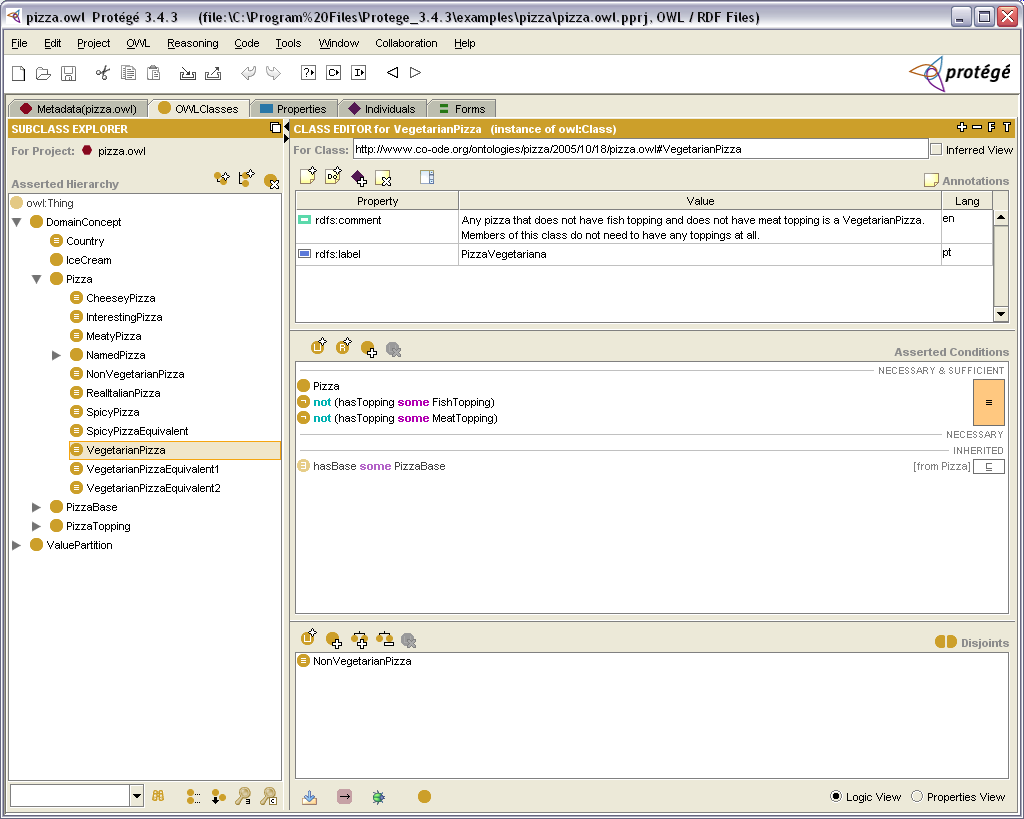
\includegraphics[width=12cm]{Protege_3.png}
    \caption{Tela Principal do Software Protégé}
    \label{fig:Protege343}
\end{figure}

O Protégé\footnote{http://protege.stanford.edu/products.php} é um software livre (opensource), com estrutura para a construção de sistemas inteligentes.

Sua interface é baseada em formularios (\autoref{fig:Protege343}), e portanto mais complexa de se trabalhar. Apesar da interface necessitar de um conhecimento mais aprimorado, os recursos oferecidos pelo Protégé não são encontrados em outros softwares.

Para poder utilizar esta ferramenta, é necessário sua instalação no computador.

\section{WebVOWL}
O VOWL\footnote{http://www.http://vowl.visualdataweb.org/} é uma linguagem visual bem especificada para a representação orientada para o utilizador de ontologias. Ele define representações gráficas para a maioria dos elementos do Web Ontology Language (OWL), que são combinados para um layout gráfico direcionado, visualizando a ontologia (\autoref{fig:WebVOWL}). Em contraste com trabalhos relacionados, VOWL aponta para uma representação intuitiva e abrangente que também é compreensível para os usuários menos familiarizados com ontologias. Ele é um aplicativo independente inteiramente baseado em padrões web abertos. 


\begin{figure}[h]
    \centering
    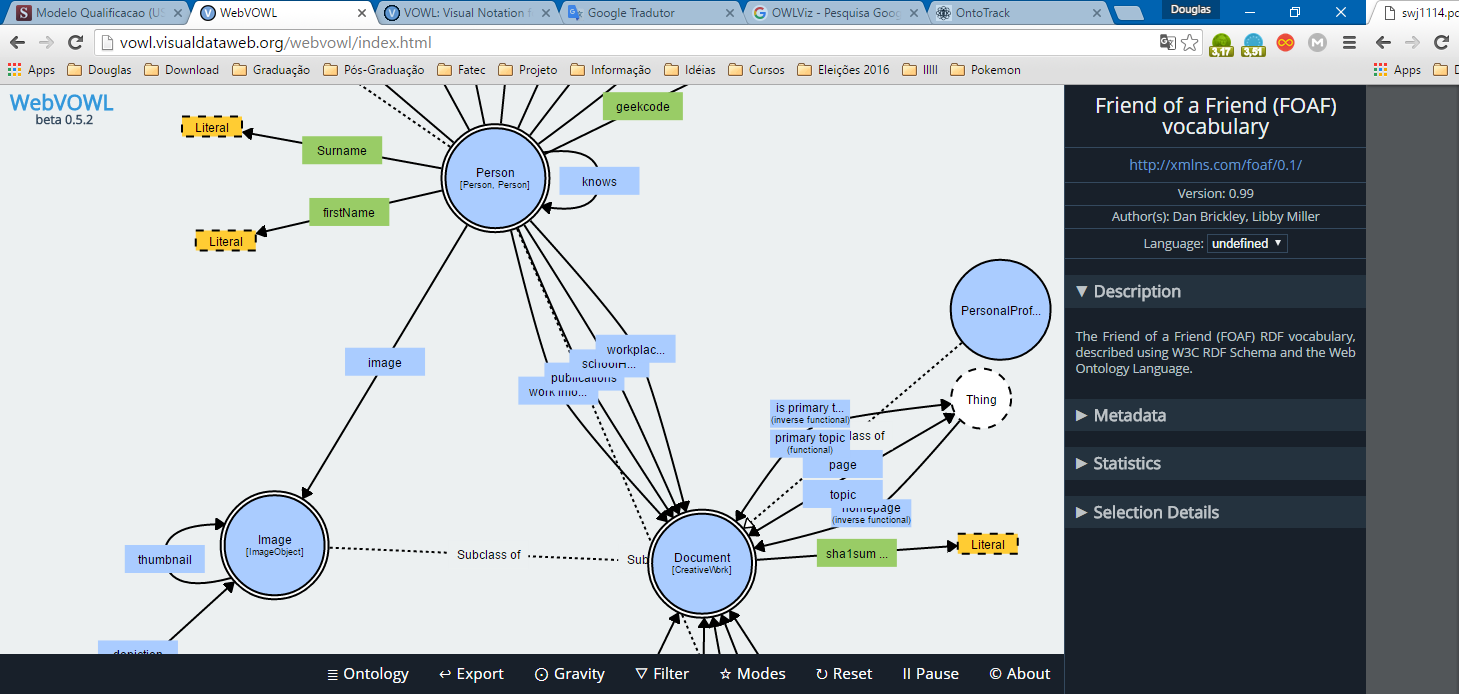
\includegraphics[width=12cm]{WebVOWL.png}
    \caption{Tela Principal do Software WebVOWL}
    \label{fig:WebVOWL}
\end{figure}

O VOWL serve unicamente como visualizador de ontologia em formato de grafos, não sendo possivel sua edição. Outra situação, no VOWL é que também não é possivel a resolução da ontologia (RESORNER), pois o mesmo não tem tal recurso.

\section{OntoTrack}

Na \autoref{fig:OntoTrack}, é demonstrada a interface do software OntoTrack. Como pode-se observar ele não é web e portanto existe a necessidade de se instalar o aplicativo no computador. Outra caracteristica é que apesar da instalação, existem versões para os sistemas operacionais mais utilizados hoje (Windows, Linux, MacOS e SunOS). Após instalado ele ira ocupar aproximadamente 8 mb de espaço, o que não tem um peso muito grande nos equipamentos atuais.

A importação de arquivos para o OntoTrack assim como a exportação, usa o parser RDF Jena2 \cite{McBride2001}. O modelo de ontologia interna da Jena2 de classes e propriedades também serve como modelo de representação central para o OntoTrack. Atualmente, OntoTrack é capaz de ler e escrever ontologias OWL Lite. No entanto, as propriedades, bem como propriedade global, restrições (declarações de domínio e alcance) não são editáveis no OntoTrack no momento.

\begin{figure}[h]
    \centering
    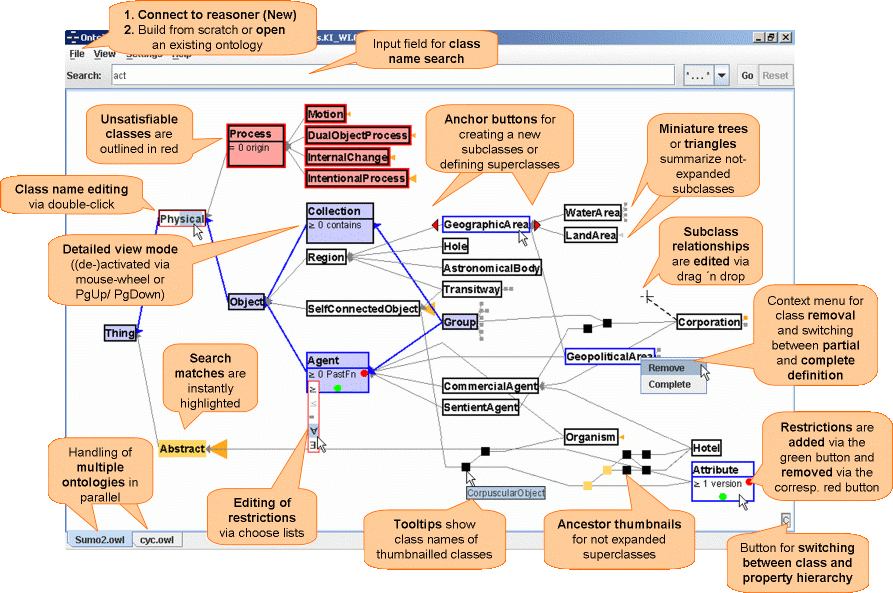
\includegraphics[width=12cm]{OnTrack.png}
    \caption{Tela Principal do Software OntoTrack}
    \label{fig:OntoTrack}
\end{figure}


\section{OWLViz}

O OWLViz é projetado para ser usado com o editor Protege-OWL. Ele permite hierarquias de classe em uma Ontologia OWL para ser visto e incrementalmente navegado, permitindo a comparação da hierarquia de classes afirmada e a hierarquia de classe inferida. O OWLViz integra com o editor Protege-OWL, utilizando o mesmo esquema de cores de modo que as classes primitivas e definidas podem ser distinguidos, mudanças computados para a hierarquia de classes pode ser visto claramente, e os conceitos inconsistentes são destacadas em vermelho, tem a facilidade para salvar ambos os pontos de vista afirmados e inferidos da hierarquia de classes para vários formatos gráficos, incluindo PNG, JPEG, e SVG.

Na \autoref{fig:OwlViz} pode ser visto a tela principal do Protege-OWL com o uso do plugin OWLViz. Assim como o Protégé, é necessário a instalação deste plugin no computador, alem disse, tem que se observar a versão do plugin se é compativel com a versão do Protégé instalada. Caso faça atualização no software Protégé, este plugin terá que ser atualizado também.

\begin{figure}[h]
    \centering
    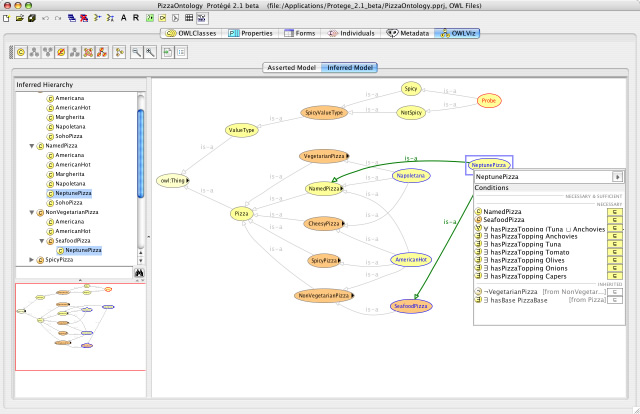
\includegraphics[width=12cm]{OwlViz.jpg}
    \caption{Tela Principal do Software Protégé com o Plugin OWLViz}
    \label{fig:OwlViz}
\end{figure}


\section{Conciderações Finais}

Apesar de existir ferramentas para elaboração de ontologias e para sua visualização em formato de grafos, não foi localizado nenhuma ferramenta que tenha suporte satisfatório aos dois tipos, podendo inclusive mudar a visualização de acordo com o especialista que trabalho com o sistema.